\chapter[数分/高代在学什么?]{
  \begin{center}
      \textbf{\LARGE {数分/高代在学什么?}}\\
      {\itshapeCJK \normalsize{食人妖怪}}
  \end{center}
 }
\addauthor{食人妖怪}

数学分析和高等代数,是每一位数学专业的新生一上来就要面对的两门课程。在这两门课程里,一切都要以严格的数学语言表达,但这些冷酷的字句后面,往往有着简单直接的想法作为直接支撑。

遗憾的是,由于教学顺序上的不合理和教材叙述的不足,这些简单直接的想法很多时候被隐藏了。这就造成了新生学习上的困难:用意义不明的符号作着莫名其妙的计算,为不知所谓的结论给出胡言乱语的证明……

通过这篇文章,我们希望尽可能简单地介绍这些课程内容背后的想法动机。我们不会给出严肃的证明,但偶尔会勾勒其想法。尽管阅读本文不能替代正经的课程学习,但或许能把你暂时变成一个“云玩家”,使你能够了解这些东西有多么好玩。
\section{数学分析}

作为一篇介绍性质的文章,我们在此仅介绍一元微积分学中的一些想法直观。多元微积分学的很多内容,都可以和一元微积分学比照学习。受限于篇幅,我们不可能面面俱到地提及全体概念,对课程的学习和思考仍是不可少的。
\subsection{实数定义,极限与连续}

我们早已接触并频繁使用实数,但实数是什么?大部分人第一次接触到的定义是“实数是有限小数和无限小数”。可是,我们只知道有限个数的加法,凭什么无穷多个数码能定义出一个无限小数呢?尽管我们能进行一些想象,但可能很难用严格的数学语言描述“无限小数”是什么。

在数学里,一切都要有严格、精确的定义。因此,
我们的第一个任务,就是合理地定义实数。

假设你已经熟知了整数的性质。通过考虑“两个数相除(分母非$0$)”,我们可以得到有理数。在有理数上,我们有四则运算,还有一个大小关系。

通过这个大小关系,我们可以暂时抛开严谨性,进行一些直观的想象。可以想象全体有理数“排列在一条直线上”。尽管有理数是“稠密”的——直线上每一小段“开区间”内都含有有理数,但是有理数之间还是有一些“间隙”,比如这个经典的例子:“长为$1$的正方形的对角线长”。

\begin{center}
    \begin{tikzpicture}[scale = 3]
        \draw[->] (-1.2, 0) -- (2.2, 0);
        \foreach \x in {1,...,10}
            {
                \filldraw (1/\x, 0) circle(0.01);
            }
        \filldraw[fill = white] (1.41421, 0) circle(0.01);
        \filldraw (2/3, 0) circle(0.01);
        \filldraw (2, 0) circle(0.01);
        \filldraw (-1, 0) circle(0.01);
        \coordinate[label = below:{\footnotesize\(\sqrt{2}\)}]() at (1.41421, 0);
        \coordinate[label = below:{\footnotesize\(2\)}]() at (2, 0);
        \coordinate[label = below:{\footnotesize\(1\)}]() at (1, 0);
        \coordinate[label = below:{\footnotesize\(\frac{1}{4}\)}]() at (0.25, 0);
        \coordinate[label = above:{\footnotesize\(\frac{1}{3}\)}]() at (1/3, 0);
        \coordinate[label = above:{\footnotesize\(\frac{2}{3}\)}]() at (2/3, 0);
        \coordinate[label = above:{\footnotesize\(\frac{1}{2}\)}]() at (0.5, 0);
        \coordinate[label = below:{\footnotesize\(0\)}]() at (0, 0);
        \coordinate[label = below:{\footnotesize\(-1\)}]() at (-1, 0);
        \coordinate[label = above:{\footnotesize\(\cdots \)}]() at (1/6, 0);
    \end{tikzpicture}
\end{center}


怎么利用有理数找到并精准地描述这些“坑”呢?Dedekind 的想法是利用“分划”:将有理数集划分为两个集合$A,B$,使得“下集合”$A$中的任一数比“上集合”$B$中全体数都小。此时我们称$(A,B)$定义了一个实数,也就是“夹在$A$和$B$中间”的那个实数。为了避免不同的分划定义同一个实数,我们进一步要求$B$中没有最小数。这样,实数集就可定义为满足上述条件的有理数划分$(A,B)$构成的集合。

有了实数集之后,可以定义我们想要的大小关系和运算:大小关系可以用分划中下集合的包含关系定义,两个元素$(A,B)$,~$(A',B')$的加法则可定义为$(A+A',B+B')$,其中
\[S+T=\left\{ \,s+t\mid s\in S,t\in T\, \right\} ,\]
容易验证相加得到的是一个分划。乘法可以类似地定义,但要小心处理一下正负号。

这种定义实数的方式比较直观,但是没有解释什么是“无限小数”。接下来我们换一种方式定义实数。我们先来看一看之前所说的“无限小数”有怎样的特征:考虑无限小数$3.1415926\cdots$,考虑一列有限小数:
\[3.14,\quad3.141,\quad3.1415,\quad3.141592\cdots.\]
这一列数虽然一直在增加,但是可以想象这列数最后会“趋向”我们尚未定义的无限小数。这是因为这列数“摆动”的幅度在减小。数列中第一项以后的任一项和第一项的差值不超过$0.01$,第二项以后任一项和第二项的不超过$0.001$……以此类推。无论给出多么小的一个“幅度”$\varepsilon$,我们都可以找到某个$N$,使得在第$N$项后任两项的差的绝对值都不会超过这个幅度$\varepsilon$。我们将这个特征推广到一般的有理数列$\{a_n\}$,用严肃的数学语言\footnote{“$\exists$”相当于“存在”,“$\forall$”相当于“对于任意的”。}描述如下:
\[\forall \varepsilon>0,\,\exists N,\,\forall  m,n\geqslant  N,\,|\,a_m-a_n|\leqslant  \varepsilon.\]
我们将这样的数列称为Cauchy列,定义里用到的就是所谓的$\varepsilon$-$N$语言\footnote{在我们定义出实数之前,$\varepsilon$只能是有理数。但我们定义出实数之后,$\varepsilon$可以在实数中取值。}。此时我们称数列$\{a_n\}$定义了一个实数,也就是直观上$\{a_n\}$“逐渐靠近”的那个实数。

当然,两个数列可能会靠近“同一个数”。比如常值数列$\{0\}$和数列$\{ 1/n\}$。直观上,这两个数列都是“逐渐靠近$0$”的。因为给定一个幅度$\varepsilon$,都存在一个$N$,使得在$N$项之后,每一项与$0$的差的绝对值不会超过$\varepsilon$。我们可以继续使用$\varepsilon\text{-}N$来定义这件事:称数列$\{a_n\}$收敛至$a$或$a$是$a_n$的极限,如果
\[\forall \varepsilon>0,\,\exists N,\,\forall n\geqslant  N,\,|\;\!a_n-a|\leqslant  \varepsilon.\]
我们将其记为
\[\lim a_n=a.\]
称两个Cauchy列$\{a_n\}$,~$\{b_n\}$定义同一个实数,
当且仅当$\{a_n-b_n\}$收敛至$0$。我们也可以在如此定义的实数集合上定义四则运算和大小关系,篇幅所限不再赘述。

刚刚对数列收敛和极限的定义,也可以对实数数列进行。在实数上,收敛于某个实数的数列和Cauchy列是完全等价的。可以证明,极限可以和基本的四则运算交换:
\[
    \lim(a_n+b_n)=\lim a_n+\lim b_n,\quad\lim(a_n\cdot b_n)=\lim a_n\cdot \lim b_n,
\]
\[\lim b_n\neq 0,\quad\lim \frac {a_n}{b_n}=\frac{\lim a_n}{\lim b_n}.\]
只要等式右侧的所有极限存在。

数列$\{a_n\}$的极限可以看作$n$走向“无穷大”时,对数列状态的描述。有时我们会使用记号$+\infty$和$-\infty$指代正的“无穷大”和负的“无穷大”。需要注意的是,这两者并不在我们定义的实数之内,我们没有赋予其任何意义。因此,我们一般不会让$\pm\infty$参加可能引起歧义的运算,但也可以定义数列$\{a_n\}$数列“趋于”$+\infty$(或相应地,$-\infty$):若
\[\forall  M>0,\,\exists N,\,\forall n\geqslant  N,\,a_n\geqslant  M,\]
则称$\{a_n\}$趋于$+\infty$。

通过数列极限,我们可以定义怎样对无穷多个数“求和”:对数列$\{a_n\}$如果部分和的序列$A_n=a_1+\cdots +a_n$收敛于$A$,则称$A$是数列$\{a_n\}$的和。此时我们也说,级数
$\sum_{n=1}^{+\infty}\,a_n$
收敛。

一般来说,无穷求和不能保证项之间可以随意交换,比如
$\sum_{n=1}^{+\infty}\,\dfrac{(-1)^{n-1}}{n}$
是收敛的,但如果将求和中的项重新排序,新得到的级数和可以收敛到任何一个实数,也可能根本不收敛。其原因在于级数的“总振幅”
\[\sum_{n=1}^{+\infty}\,\left|\dfrac{(-1)^{n-1}}{n}\right|=\sum_{n=1}^{+\infty}\,\dfrac{1}{n}.\]
是趋于正无穷的\footnote{这个结论称为Riemann重排定理。}。如果
$\sum_{n=1}^{+\infty}\,|a_n|$
是收敛的,我们称级数$\sum_{n=1}^{+\infty}\,a_n$
绝对收敛。此时级数的项可以随意交换顺序。

数列可以看作定义在正整数上的“函数”。因此除了考虑数列的极限,我们还可以考虑一般的函数的极限。函数极限的种类要更丰富:不仅有自变量趋于正无穷/负无穷时的极限,还有趋于某个实数$x_0$时的极限。前两者和数列的情形大同小异,值得注意的是后一种情形:设有实数$a$和函数$f$,如果$f$在$x_0$周围——或者说,$x_0$的某个“邻域”$(x_0-h,x_0+h)$上有定义,且
\[\forall \varepsilon>0,\,\exists \delta>0,\,\forall x,\,0<|x-x_0|\leqslant  \delta,\,\bigl|\,f(x)-a\bigr|\leqslant  \varepsilon,\]
则称$a$是函数$f$在$x$趋于$x_0$处的极限,记为
\[\lim_{x\to x_0}f(x)=a.\]

在这个定义里面,如果将对$x$的要求从$|x-x_0|\leqslant  \delta$改成$x_0<x\leqslant  x_0+\delta$,即只在$x_0$的右侧变动,则称$a$是$f$在$x_0$的右极限。完全类似地,也可定义左极限。我们分别使用记号
\[\lim_{x\to x_0^+},\quad \lim_{x\to x_0^-}.\]

细看函数极限的定义,可以发现$x$不能取$x_0$。这是因为我们希望研究函数在$x_0$周围的性状,但函数本身在$x_0$可能有定义,所以需要排除掉函数在$x_0$的取值对周围性状的影响。比如下面的函数:
\[f(x)=
    \begin{dcases}
        0, & x\neq 0; \\
        1, & x=0.
    \end{dcases}
\]
$f$在$0$周围的取值都是$0$,但是$f(0)=1$。按照定义,此时函数在$0$处的极限是$0$而非$1$。

\begin{center}
    \begin{tikzpicture}[scale = 1.5]
        \draw[->] (-3.2, 0) -- (3.2, 0);
        \draw[thick] (-3.2, 0) -- (3.2, 0);
        \draw[->] (0, -1) -- (0, 2);
        \filldraw[fill = white, thick] (0, 0) circle(0.03);
        \filldraw[thick] (0, 1) circle(0.03);
        \coordinate[label = -135:{\(0\)}]() at (0, 0);
        \node[]() at (0.5, 0.5){\footnotesize\(f(0)=1\)};
    \end{tikzpicture}
\end{center}

直观上看,这种现象的出现是由于$f$的图像在$0$处“断掉了”。我们可以以此定义函数的“连续性”:
设函数$f$在$x_0$的某个邻域$(x_0-h,x_0+h)$上有定义,同时
\[\lim_{x\to x_0}f(x)=f(x_0),\]
则称$f$在$x_0$连续;

如果$f$在某个开区间$I$(特别地,$I$可以取成全体实数)上有定义且在$I$中每一点连续,则称$f$在$I$上连续;

至于闭区间,我们只要在端点处用相应的单侧极限代替极限,就可以得到闭区间上连续函数的定义。

“连续”是一个基础而重要的概念,值得反复探讨。首先,根据连续性的定义,每一个局部的“连续”可以决定整体的连续。其次,我们可以用“小片”上的连续函数“粘”出“大片”上的连续函数:设开区间$I$可以分解为一些小开区间$I_j$之并。如果对每个$I_j$分配一个$I_j$上的连续函数$f_j$,使得在任两个区间$I_j$,~$I_{j'}$重叠的部分,$f_j$,~$f_{j'}$的取值也相同。那么我们可以得到一个$I$上的连续函数$f$。反过来,$I$上的连续函数$f$也可以将定义域限制在每个开区间$I_j$上,得到一族连续函数$f_j$。这种限制与粘合的构造是许多数学概念的源头。

从直观上看,连续就是“不断”。如果一个画在$xOy$平面上的函数一部分在$x$轴以上,一部分在$x$轴以下,那么一定要和$x$轴相交——这就是连续函数的介值定理,可以用来证明某些方程的解存在。

我们可以回头看一看我们是如何定义出连续的,这主要依赖于我们对“距离”的刻画——绝对值函数$|x-y|$。在某些场合,我们处理的“函数”不再是定义在实数上的,如果此时我们仍能定义一个满足一定条件的“距离”,我们依然可以讨论连续性。

但即使是这个条件,有时也显得过于苛刻。我们可以干脆将“距离”也抛弃掉,转而使用“邻域”来刻画连续性:设$f:X\to Y$,设$x_0\in X$,如果对$f(x_0)$不论多么“小”的邻域$V$,都可以找到$x_0$的一个“小”邻域$U$,使得$f$将$U$整个映到$V$内部,那么就称$f$在$x_0$连续。我们只需要给出“邻域”的足够精当的描述,这正是点集拓扑的内容。数学分析里的不少内容,都能看出点集拓扑学的影子。如果你学有余力,学一些点集拓扑的帮助是很大的。
\subsection{导数和积分}

我们在高中的时候介绍过导数的概念,当时我们使用的是“切线”的几何直观。现在,我们以“逼近”的角度来重新认识导数。

贯穿分析学的一个想法是“以好对象逼近坏对象”。因此对一些性质较好的函数,我们可以尝试在某一点$x_0$附近以“线性函数”进行逼近。这个一次函数的斜率就是我们说的导数$f'(x_0)$,其定义为
\[f'(x_0)=\lim_{x\to x_0}\dfrac{f(x)-f(x_0)}{x-x_0}.\]
在$x_0$点附近,对于一个很小的增量$\Delta x$,函数值$f(x_0+\Delta x)$可以被线性函数$f(x_0)+f'(x_0)\cdot\Delta x$逼近。

对两个函数$f$,~$g$,在$x_0$附近我们将$f$,~$g$分别用相应逼近的线性函数代替,作加法、乘法\footnote{我们在得到的结果中舍去$(x-x_0)^2$项,因为它比$x-x_0$衰减地更快。}、复合,就可以看到导数之间的关联:
\[\bigl(\,f+g\bigr)'(x_0)=f'(x_0)+g'(x_0),\quad\bigl(\,fg\bigr)'(x_0)=f'(x_0)g(x_0)+f(x_0)g'(x_0),\]
\[\bigl(\,f\circ g\bigr)'(x_0)=f'(g(x_0))g'(x_0).\]

某种意义上,这是“最佳”的逼近。根据极限的四则运算,
\[\lim_{x\to x_0}\dfrac{f(x)-f(x_0)-f'(x_0)(x-x_0)}{x-x_0}=0.\]
也就是说,误差项$f(x)-f(x_0)-f'(x_0)(x-x_0)$在$x_0$附近“衰减”地比线性函数更快。我们已经不能通过调整一次项的系数,使误差在$x_0$周围减小地更快了。

为了进一步捕捉误差,我们可以使用衰减更快的项$(x-x_0)^k$,即用多项式函数来逼近$f$。当函数$f$的性质足够好时,我们有Taylor展开:

\begin{align*}
    f(x) & =  f(x_0)+\frac{f'(x_0)}{1!}(x-x_0)+\frac{f''(x_0)}{2!}(x-x_0)^2+\frac{f^{(3)}(x_0)}{3!}(x-x_0)^3 \\
         & \mathrel{\phantom{=}}+\cdots+\frac{f^{(n)}(x_0)}{n!}(x-x_0)^n+R_{n+1}.
\end{align*}


其中$f^{(n)}=\left(\, f^{(n-1)} \right)'$,~$\,f^{(1)}=f'$,$R_{n+1}$是一个比$(x-x_0)^n$衰减更快的余项。这个展式可以帮助我们计算很多奇怪的极限,但将大量的时间花费在这种计算上未必是明智之举。


积分的想法则来源于计算“面积”——尽管我们并没有定义什么是面积。按照我们朴素的想法,矩形的面积应该等于邻边相乘,同时面积应当具有某种“可加性”。于是对曲线下方图形的面积,我们可以尝试用一列矩形进行逼近。比如对定义在闭区间$[a,b]$上的函数$f$,我们可以选取矩形端点落在$x$轴上的位置分别是$a=x_0<x_1<\cdots  <x_n=b$。同时,我们选取每个矩形的“高度”:一种取法是在小段$[x_{i-1},x_{i}]$里面任意地选取一点$\xi_i$,将$f(\xi_i)$作为矩形的高。这样选取之后,计算出来小矩形的面积和\footnote{当然,$f$可以取负值。此时我们寻求的“面积”并不是直接的“面积”,而是指“带符号的面积”,即在$x$轴上方的部分和$x$轴下方部分面积的差值。}就是:
\[\sum_{i=1}^n  \,f(\xi_i)(x_i-x_{i-1}).\]

当然,上面的和式和我们真正需要的面积会有一定的“差距”,这些差距来源于矩形和曲线之间的部分。直观上看,如果我们的矩形的宽能够都选得更小,那么这些矩形和曲线就会“贴得更近”,得到的误差也会更小。

利用之前学习的经验,我们用$\varepsilon\text{-}\delta$语言来叙述这件事:如果存在实数$A$,对于任意的$\varepsilon>0$,都存在$\delta>0$,使得各个区间$[x_{i-1},x_i]$的长度均不超过$\delta$时,无论$\xi_i$如何选取,总有
\[\left|\,\sum_{i=1}^n  \,f(\xi_i)(x_i-x_{i-1})-A\,\right|\leqslant  \varepsilon.\]
那么我们称$A$是函数$f$在区间$[a,b]$上的定积分,记为
\[\int_a^{b} \,f(x)\,\mathrm{d}x.\]

定积分的存在通常需要一些具体的条件来保证,比如函数在闭区间上连续。通过定积分,我们可以为一些比较“规整”的图形定义面积,满足区域可加性并且符合我们以往的认知。

一个意外之喜是,通过积分我们可以发现求导数的“逆运算”。设$f$在全体实数上有定义且连续,固定一点$a$,我们考虑
\[F(x)=\int_{a}^x\,f(t)\,\mathrm{d}t.\]
其中$x$是$F$的变量\footnote{当$x<a$,我们定义$F(x)$为$f$在$[x,a]$上定积分的相反数,因为我们改变了方向。},而$t$是积分使用的变量。

当$x$在$x_0$处产生一个小增量$\Delta x$时,可以想象,“增加的面积”可以被宽为$\Delta x$,高为$f(x_0)$的小矩形逼近。结合我们之前有关导数“线性逼近”的介绍,可以发现此时$F'(x_0)=f(x_0)$。这样,我们就找到了一个函数$F$,使得$F'=f$。由于常函数求导为$0$,$F$加上任何一个常数都满足同样的性质\footnote{这也能说明为什么我们可以任意地选取起点$a$。}。

反过来,如果我们找到了一个函数$F$,$F'=f$,那么它和我们之前寻求的定积分相差某个常数。这是我们计算定积分的一个重要的依据,也就是著名的牛顿-莱布尼兹公式:
\[\int_a^b\,f(x)\,\mathrm{d}x=F(b)-F(a).\]
我们可以拿这个公式算出许多我们关心的面积。

按我们上面定义积分的方式,被积函数$f$是不能和连续函数相差太远的\footnote{相应的结论是黎曼-勒贝格定理。}。这给我们定义“面积”带来了一定的限制。我们可能会遇到长相千奇百怪,极不规整,相当“丑陋”的点集,这时用矩形去逼近面积是完全不可能做到的,上面做出的种种努力也都失效了。

为此,我们要回到“面积”的本质——可加性上面,小心地探讨何时可以“定义面积”,怎样用面积得到函数的“积分”,又有哪些函数可以计算积分……这就是测度论所研究的内容了。你可能会在后续的实分析课程上见到这些,并且重建一套被称为Lebesgue积分的新积分体系——但对初学者而言,最好还是从这些基础内容脚踏实地地学起。
\subsection{函数列与函数级数}
之前我们定义了数列的极限,并以此定义了数项级数的求和。完全类似地,如果我们将数列的每一项换成关于某个变量$x$的函数$f_n(x)$,就可以得到相应的函数列和函数项级数。

如果对每个$x$值,相应的数列$f_n(x)$或级数$\sum_{n=1}^{+\infty}\,f_n(x)$收敛,我们就称函数列(函数级数)逐点收敛。为了方便,我们暂且讨论函数列的收敛,函数项级数的收敛是完全类似的。

对每个$x$,记$f_n(x)$的极限为$f(x)$,这是一个新的函数。通常来说,我们取的$f_n$是熟知的、性质较好的函数,但其极限$f$是我们了解较少的对象。我们要问,能否从$f_n$的性质推知$f$的性质?如果可以,我们就可以通过对研究“好函数”$f_n$得到“坏函数”$f$的性质。

我们先从相对比较简单的连续性入手。如果$f_n$都是连续的,可以推出$f$是连续的吗?很容易发现如下的反例:取$[0,1]$上的函数$f_n(x)=x^n$,则其极限为
\[f(x)=
    \begin{dcases}
        0, & 0\leqslant  x< 1; \\
        1, & x=1.
    \end{dcases}
\]
很明显不是连续函数。

为什么$f$会在$1$附近断开?当$x\in(0,1)$逐渐靠近$1$时,$f_n(x)$虽然总是收敛于$0$的,但其收敛的“速度”会越来越慢。无论对多么大的正整数$N$,在$x=\dfrac {1}{\sqrt[N]{2}}$处,$f_N(x)$的值都是$\dfrac 12$而与$0$相距甚远。

这个现象告诉我们,对函数列而言,除了逐点的收敛性,我们还要关注“不同$x$之间”的收敛速度会不会相差太远。我们以此定义一致收敛的概念:对函数列$\{\;\!f_n\}$,若
\[\forall \varepsilon>0,\,\exists N,\,\forall n\geqslant  N,\,\bigl|\,f_n(x)-f(x)\bigr|\leqslant  \varepsilon,\,\forall x,\]
则称函数列$\{f_n\}$一致收敛至$f$.

虽然这个定义乍一看和数列极限区别不大,但其精髓在于$N$ 无关$x$的选取。我们可以比较逐点收敛的叙述:
\[\forall x,\,\forall \varepsilon>0,\,\exists N,\,\forall n\geqslant  N,\,|\,f_n(x)-f(x)|\leqslant  \varepsilon.\]
两者虽然形式上极度相似,但表达的含义是截然不同的。

在相应的函数列一致收敛\footnote{注意到,命题在更弱的条件下依然成立:相应的函数列在每一个子闭区间内一致收敛。比如在全体实数上收敛的幂级数,通常就不是一致收敛的,但在子闭区间$[-M,M]$上,我们可以用$M$进行控制。}的设定下,我们也可以通过$f_n$的导数或积分得到$f$的导数或积分。如果$f_n'$一致收敛,则
\[f'(x)=\lim f_n'(x).\]
如果$f_n$一致收敛,则
\[\int_a^b\,f(x)\,\mathrm{d}x=\lim \int_a^b\,f_n(x)\,\mathrm{d}x.\]
形式上,这些操作相当于“交换极限和导数/积分”。通常来说,这种交换次序的操作都需要某种一致性来保证。

现在,我们可以用函数列/函数项级数来研究函数。之前我们提到,性质好的函数可以用多项式逼近。为了扔掉难以捉摸的余项,我们自然希望可以“无限地”展开下去:
\[f(x)=f(x_0)+\frac{f'(x_0)}{1!}(x-x_0)+\frac{f''(x_0)}{2!}(x-x_0)^2 +\cdots+\frac{f^{(n)}(x_0)}{n!}(x-x_0)^n+\cdots\, .\]
这促使我们研究形如$\sum_{n=1}^{+\infty}\,a_nx^n$的幂级数。我们可以研究其在怎样的区域内收敛或一致收敛,是否收敛于我们想要的函数,等等。

可以证明,幂级数$\sum_{n=1}^{+\infty}\,a_nx^n$会在某个以原点为中心,半径$r$(可能为$0$或$+\infty$)的圆盘 内部绝对收敛,在外部发散,而在边界圆周上则既可能收敛,又可能发散。比如下面两个幂级数
\[\sum_{n=0}^{+\infty}x^n=\frac 1{1-x},\quad \sum_{n=0}^{+\infty}(-1)^nx^{2n}=\frac{1}{1+x^2}.\]
都仅在$|x|<1$时收敛。前者很容易理解,是由于函数在$1$附近的奇异性。但后者该作何解释?只有把关心的范围从实数扩大到复数,并对复变量的函数定义极限、导数、积分这些概念,才能得到令人满意的解释。而这一切都将会是复分析学习的内容。

\section{高等代数}
我们即将学习的代数学,并不仅仅是中学数学中的简单计算。粗略地讲,我们希望研究集合上的各种代数结构。按常见的课程划分,“线性代数”和“抽象代数”是这方面比较基础的两门课程。

虽然这两门课被安排在不同的阶段,但其内容之间是紧密关联的。而“高等代数”课程的定位通常介于这两者之间,是在线性代数的基础上加一点点抽象代数的内容。
本文主要介绍线性代数的内容,但也会体现一些抽象代数的观点。
\subsection{“结构”与线性空间}
我们高中就接触过简单的集合论。不严谨的说,集合就是一堆“元素”构成的一个整体。设有集合$A$,~$B$,如果我们对集合$A$中每一个元素$a$都按某种法则指定一个确定的$B$中元素$f(a)$,我们就得到从$A$到$B$的一个映射$f$。如果对每一个元素$a\in A$,有且仅有一个$b\in B$使得$f(a)=b$,我们称$f$是双射或一一对应。此时有逆映射$f^{-1}:B\to A$,使得$f^{-1}\bigl(\,f(a)\bigr)=a$。

虽然集合已经是相当基本的数学对象,但仅有集合是不够的。举例而言,我们所说的“自然数”实际上要比“自然数集”多出了不少信息。在一个集合里,元素之间通常是“没什么关系”的,但“自然数”并非如此。自然数之间可以进行运算和比较,比如我们熟知的加法、乘法和大小关系。正整数相加、相乘的结果不会跑出正整数集,所以加法和乘法两种运算实际上都是映射\footnote{对集合$A$,~$B$,定义Descartes积$A\times B$为其元素的有序对组成的集合:$\{(a,b)\mid a\in A,b\in B\}$。
}:$ \mathbb{N}\times\mathbb{N}\to \mathbb{N}$。而大小关系$\leq$实际上是$\mathbb{N}\times\mathbb{N}$满足某些条件的一个子集,$(x,y)$在这个子集中当且仅当$x\leqslant y$。这些额外的“信息”就可称为自然数集合上的“结构”。

现在我们考虑大一些的数集,比如有理数集$\mathbb{Q}$。由于有理数对加法和乘法封闭,加法和乘法都是$\mathbb{Q}\times\mathbb{Q}\to\mathbb{Q}$的映射,满足我们熟知的交换律、结合律以及乘法对加法的分配律。$0$和$1$分别是加法、乘法的“单位元素”,这就是说对任意$x\in\mathbb{Q}$,
\[0+x=x+0=x,\quad 1\cdot x=x\cdot 1=x. \]

每个元素$x\in\mathbb{Q}$都有加法逆元,即存在元素$-x$,使得\[-x+x=x+(-x)=0.\]每个$\neq 0$的元素$x$都有乘法逆元,即存在元素$\dfrac 1x$,使得\[x\cdot \dfrac{1}{x}=\dfrac{1}{x}\cdot x=1.\]实数集$\mathbb{R}$、复数集$\mathbb{C}$也都有完全一样的性质。我们将包含$\mathbb{Q}$且满足上述条件的$\mathbb{C}$的子集称为数域。通俗地说,数域就是对加减乘除(除数非$0$)都封闭的数集。在数域里,我们可以随意地进行四则运算而不必担心超出我们考虑的范围。

我们高中还接触过“向量”的概念。在平面$\mathbb{R}^2$上,始于原点的向量按照终点的位置和$\mathbb{R}^2$上的点一一对应。通过这个对应,我们对向量进行的一切操作可以视同对$\mathbb{R}^2$内的元素进行。我们回忆几个操作:

向量加法:对$(a,b)$,~$(c,d)\in\mathbb{R}^2$,$(a,b)+(c,d)=(a+b,c+d)$。这个加法满足交换律、结合律,且有零向量$(0,0)$作为加法的单位元素,每个向量$v$都有加法逆元$-v$。

向量数乘:对$(a,b)\in\mathbb{R}^2$和$k\in\mathbb{R}$,有$k (a,b)=(ka,kb)$。这是一个映射:$\mathbb{R}\times\mathbb{R}^2\to\mathbb{R}^2$,同样满足某种意义上的“结合律”和“分配律”:对$v$,~$v'\in \mathbb{R}^2$,$k$,~$k'\in\mathbb{R}$,我们有
\[k(v+v')=kv+kv',\quad (k+k')v=kv+k'v,\quad k(k'v)=(kk')v,\quad 1v=v.\]

我们将这个结构提炼出来,就可以得到线性空间的概念:

设$F$是一个数域,$V$是一个集合,定义了一个加法$V\times V\to V$和一个数乘$F\times V\to V$,使得上述条件均满足,就称$V$是数域$F$上的线性空间或向量空间。

需要注意的是,线性空间是架在集合上的结构。一个集合上可以赋予不同的运算,使其成为不同的线性空间。原则上,当我们谈及某个具体的线性空间时,必须明确集合上配备了什么运算。但当运算容易从上下文中看出时,我们常常略去这一点。

我们在定义中对底集合没有任何的要求,因此可以在各种各样的集合上建立起线性空间的结构。正是这种定义上的广泛性,赋予了线性代数理论强大的生命力。我们来看几个例子:

平面上的向量(视同$\mathbb{R}^2$)按我们刚刚所说,是$\mathbb{R}$线性空间。对“高维空间”$\mathbb{R}^n$中始于原点的向量(视同$\mathbb{R}^n$),也可以用类似的方式定义运算,从而为$\mathbb{R}^n$赋予了$\mathbb{R}$上线性空间结构。

记$C[a,b]$为非空区间$[a,b]$上全体实值连续函数的集合。那么函数的加法和乘以常值函数赋予了$C[a,b]$以$\mathbb{R}$上线性空间结构。

记系数在数域$F$上以$x$为变元的全体多项式的集合为$F[x]$,以通常多项式的加法和数乘作为运算,就赋予了$F[x]$一个$F$上线性空间结构。

考虑如下的齐次线性方程组:设$a_{ij}\in\mathbb{R}$,
\[
    \begin{dcases}
        a_{11}x_1+a_{12}x_2+\cdots+a_{1n}x_n=0, \\
        a_{21}x_1+a_{22}x_2+\cdots+a_{2n}x_n=0, \\
        \mathord{\cdots}\mathord{\cdots}        \\
        a_{m1}x_1+a_{m2}x_2+\cdots +a_{mn}x_n=0.
    \end{dcases}
\]
记其所有解$(x_1,\,\dots\,,x_n)$构成的集合为$X\subset \mathbb{R}^n$,则$X$中元素对$\mathbb{R}^n$上的加法和数乘封闭,因而有了$\mathbb{R}$上线性空间结构。

$X$本身是$\mathbb{R}^n$的子集,$X$上的线性空间结构又完全继承自$\mathbb{R}^n$。此时我们称$X$是$\mathbb{R}^n$的子空间。

上面几个例子中的对象出现在数学的不同领域中。我们再一次看到线性代数理论的重要性。

\subsection{基、线性映射与矩阵}
我们继续关注平面向量这个我们比较熟悉的例子。高中时我们曾经学过平面向量基本定理:如果$u,v$是不共线的向量,那么平面上的每一个向量都可唯一地表成$au+bv$的形式。对空间向量也有类似的结果,只是此时是三个不共面的向量。

\begin{center}
    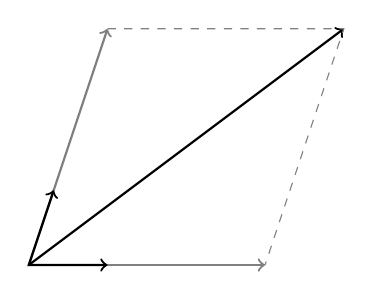
\begin{tikzpicture}
        \draw[->, thick, gray] (0, 0) -- (3, 0);
        \draw[->, thick, gray] (0, 0) -- (1, 3);
        \draw[<->, thick]  (1, 0) -- (0, 0) -- (0.316228, 0.316228 *3);
        \draw[->, thick] (0, 0) -- (4, 3);
        \draw[dashed, gray] (1, 3) -- (4, 3) -- (3, 0);
    \end{tikzpicture}
\end{center}

有了这个定理,在平面上选取了两个不共线的向量$u$,~$v$之后,所有向量就完全由两个实数$a,b$完全决定了。不难发现,我们通常使用的平面直角坐标系,实际上就是取$u=(1,0)$,~$v=(0,1)$的特殊情形。

有这样一个“坐标系”可以帮助我们解决许多问题,我们希望将其推广到任意的线性空间上。幸运的是,我们总是可以做到这一点:对任意数域$F$上的线性空间$V$,存在一族\footnote{为了方便表示,我们使用一个集合$I$中的元素作为下标,但指标集$I$可能是无穷集,也可能不可数。这里的$I$和单位矩阵没有任何关系。}元素$\{e_i\}_{i\in I}$,使得对每一个元素$v\in V$,都存在$i_1,\,\dots\,,i_n\in I$及$x_1,\,\dots\,,x_n\in I$,使得
\[v=x_1e_{i_1}+\cdots +x_ne_{i_n}.\]
同时这种表示是唯一的。此时我们称$\{e_i\}_I$是线性空间的一组基。如果$|I|$是有限的,那么两组基的元素个数是相等的,我们称其为线性空间的维数。

需要注意,我们目前只允许有限个元素进行求和,正如之前在数学分析的部分所介绍的一样。在另外,表示的“唯一性”告诉我们$e_i$之间是线性无关的。也就是说:对一切$i_1,\,\dots\,,i_n\in I$,
\[x_1e_{i_1}+\cdots +x_ne_{i_n}=0\]
当且仅当$x_1=x_2=\cdots =x_n=0$。在平面向量的情形,这相当于说两个向量不共线;在空间向量的情形,这相当于说没有一个向量落在其余两个所在的平面里。

证明向量空间都有基并不是一件简单的事情,比如对连续函数的例子,就很难想象有这样一组基存在。这个证明需要用到与选择公理等价的Zorn引理,初学者可以暂时跳过。但一旦承认了这个结果,我们的许多推理和构造都能方便许多。

接下来,我们集中关心有限维的线性空间,基中元素的个数都是有限的。

除了单独的线性空间之外,我们要在不同的线性空间之间建立起联系。设$V$,~$V'$是$F$上的线性空间,我们考虑映射$f:V\to V'$。我们希望线性空间结构能对研究起到帮助,因此我们要求$f$和线性空间结构“相容”。也即:对一切$u,v\in V$,~$c\in F$
\[f(u+v)=f(u)+f(v),\quad f(cu)=cf(u).\]
上面的等式里,左侧依赖$V$的线性空间结构,而右侧依赖$V'$的线性空间结构。我们称这样的映射为线性映射,如果$V'=V$,我们称其为线性变换,有时也称为$V$上的线性算子。

这些线性映射长什么样?我们可以在熟悉的例子里面考虑,比如平面上的线性变换。我们其实已经见过不少这样的变换:

绕原点$\theta$角的旋转。其公式为
\[(x,y)\mapsto (x\cos\theta+y\sin \theta,-x\sin\theta+y\cos\theta).\]

坐标的“伸缩”变换。对横纵坐标的比例系数$a,b\neq 0$,其规则为
\[(x,y)\mapsto(ax, by).\]

当然还有沿过原点的轴的翻转。比如:

% !
\begin{figure}[h]
    \centering
    \includegraphics[scale=0.3]{Reflection.png}
\end{figure}

这些都是线性变换的具体例子。不过,平移一般不是线性变换,因为从我们的定义容易看出线性映射将$0$映到$0$。

有了线性映射,选取基的好处就体现出来了。假如有线性空间$U,V$间的线性映射$f:U\to V$,我们选取一组$U$的基$u_1,\,\dots\,,u_n$,由于$U$中每个元素可以被$u_i$线性表出,$f$在$x\in U$的取值被$f$在$u_i$上的取值所唯一确定。

如果我们再为$V$选一组基$v_1,\,\dots\,,v_m$,那么每个$f(u_i)$又被其$v_j$分量的各个“坐标”所确定。这样,刻画这个线性映射只需要$mn$个常数$a_{ij}$,使得
\[f(u_j)=\sum_{i=1}^ma_{ij}v_i.\]
我们将这些常数排成一个$m\times n$(即$m$行$n$列)的表:
\[ A =
    \begin{pmatrix}
        a_{11} & a_{12} & \ldots & a_{1n} \\
        a_{21} & a_{22} & \ldots & a_{2n} \\
        \vdots & \vdots & \ddots & \vdots \\
        a_{m1} & a_{m2} & \ldots & a_{mn} \\
    \end{pmatrix} . \]
我们称之为线性映射$f$在基底$\{u_i\},\{v_j\}$下的矩阵。如果$f$是线性算子,我们通常取$\{v_j\}=\{u_i\}$。

线性映射的结构允许我们进行一些操作。比如两个线性空间之间的两个线性映射可以相加:\[(\;\!f+g)(x)=f(x)+g(x)=g(x)+f(x)=(g+f)(x).\]

线性映射也可以像集合的映射一样进行复合:
\[gf(x)=(g\circ f)(x)=g(f(x)).\]

容易证明这些映射都是线性的。这些线性映射之间的矩阵有何关系?

不难看出,两个线性映射$f_1$,!$f_2$的和$f_1+f_2$的矩阵是$f_1$和$f_2$的矩阵各个分量直接相加,我们称其为矩阵的和。矩阵对求和明显是交换、结合的。加法单位元是分量全为$0$的矩阵,$A$的逆元是与$A$的各个分量乘以$-1$得到的矩阵。

假设$U,V,W$分别是$m,n,p$维的线性空间,其基分别为$\{u_i\},\{v_j\},\{w_k\}$,$f,g,g\circ f$所对应的矩阵是$A,B,C$,那么$A,B,C$分别是$n\times m$,~$p\times n$,~$p\times m$的矩阵。简单的计算可以得出
\[c_{ij}=\sum_{k=1}^nb_{ik}a_{kj},\]
其中$a_{ij}$0,~$b_{ij}$,~$c_{ij}$分别是$A,B,C$在$i$行$j$列的元素。我们定义矩阵$C$为矩阵$B,A$的乘积,记为$C=BA$。映射复合的“结合律”自然给出了矩阵乘法的结合律\footnote{注意矩阵进行乘法时,前一个的列数和后一个的行数必须一致!}。在所有$n\times n$的“方阵”中,矩阵乘法的单位元是单位矩阵:
\[I=I_n=\begin{pmatrix}
        1      & 0      & \ldots & 0      \\
        0      & 1      & \ldots & 0      \\
        \vdots & \vdots & \ddots & \vdots \\
        0      & 0      & \ldots & 1      \\\end{pmatrix}.\]
但即使是对方阵,乘法也未必满足交换律。

通过上面的对应,研究映射的问题就可以被转化成研究矩阵的问题。前者往往是抽象的,而后者往往是具体而可以计算的。
\subsection{线性算子的行列式}
在$\mathbb{R}^n$里面,我们有一种对“体积”的直观感受。而$\mathbb{R}^n$上的线性算子都是“作用均匀”的拉伸变形。我们自然可以考虑一个线性算子下“体积”的变化程度。

我们以平面上的几个线性算子为例。旋转是保持面积和定向的,因此其“体积变化率”是$1$。

沿着过原点某条轴的翻转。面积的大小不变,但是其“定向”被改变了——顺时针会变成逆时针。对“有向体积”来说,这相当于改变了一个符号,因此其“体积变化率”是$-1$。

以$a$,~$b$为比例系数对进行伸缩,和之前的例子相同。此时体积变化率是$ab$。注意当$a=-1$,~$b=1$时,这相当于一个翻转;当$a=b=-1$时,这相当于一个旋转。

怎样在$\mathbb{R}^n$上计算这个体积变化率?我们选取标准基$e_i$为仅有第$i$个分量为$1$,其余均为$0$的元素。在线性算子$T$的作用下,由$e_1,\,\dots\,,e_n$“张成”的高维“立方体”会被映到$T(e_1),\,\dots\,,T(e_n)$张成的“平行多面体”:

\begin{center}
    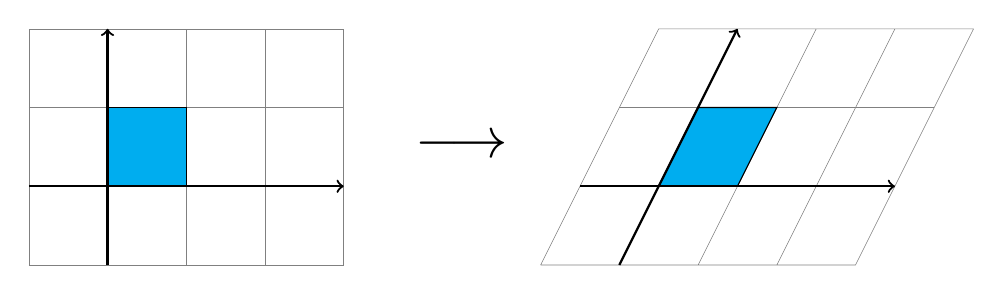
\begin{tikzpicture}
        \draw[step=1cm,gray,very thin] (-1,-1) grid (3, 2);
        \draw[fill = cyan] (0, 0) rectangle (1, 1);
        \draw[thick, ->] (-1, 0) -- (3, 0);
        \draw[thick, ->] (0, -1) -- (0, 2);

        \node at (4.5, 0.5) {\huge\(\longrightarrow\)};

        \draw[xslant = 0.5, xshift = 7cm, step=1cm,gray,very thin] (-1,-1) grid (3, 2);
        \draw[xslant = 0.5, xshift = 7cm, fill = cyan] (0, 0) rectangle (1, 1);
        \draw[xslant = 0.5, xshift = 7cm, thick, ->] (-1, 0) -- (3, 0);
        \draw[xslant = 0.5, xshift = 7cm, thick, ->] (0, -1) -- (0, 2);
        % \draw[cm={0,1,1,0,(1cm,1cm)},red] (0, 0) rectangle (1, 1);
    \end{tikzpicture}
\end{center}

我们将由始于同一点的向量$v_1,\,\dots\,,v_n$张成的平行多面体的(有向)体积记为$\mathrm{vol}(v_1,\,\dots\,,v_n)$。然而,我们还没有定义什么是“体积”!
与之前数学分析中不同,我们面对的是“平行多面体”这类简单的几何对象,中学里的几何直觉仍然发挥着一定的作用。我们按照我们“想象中”的体积提出$\mathrm{vol}$应当满足的几条性质:

首先,“单位立方体”应该具有体积$1$。因此$\mathrm{vol}(e_1,\,\dots\,,e_n)=1$。

延长某一条边会引起体积相应倍数的变化。即对$1\leqslant  i\leqslant  n$,
\[\mathrm{vol}(v_1,\,\dots\,,\,cv_i,\,\dots\,,v_n)=c\cdot \mathrm{vol}(v_1,\,\dots\,,v_n),\]
其中$c$是任意实数,可以为$0$或负数。当$c=0$,这个平行多面体被“拍扁”成了一个低维的平面,从而体积为$0$;当$c$为负值,我们改变了整个平行多面体的定向,从而体积反号。

我们知道“同底等高”的平行四边形面积是相等的。也就是说,$v_1$,~$v_2$张成的平行四边形和$v_1+c\cdot v_2$,~$v_2$张成的平行四边形面积相等。这可以推广到高维情形:对一切$1\leqslant  i,j\leqslant  n$,~$i\neq j$,
\[\mathrm{vol}(v_1,\,\dots\,,\,v_i+c v_j,\,\dots\,,v_n)=\mathrm{vol}(v_1,\,\dots\,,v_n).\]
可以证明,有了上面几条性质,函数$\mathrm{vol}$就被唯一地确定了。给定$V$上的一个线性算子$T$,可以证明当$\mathrm{vol}(v_1,\,\dots\,,v_n)\neq 0$时,
\[\frac{\mathrm{vol}(Tv_1,\,\dots\,,Tv_n)}{\mathrm{vol}(v_1,\,\dots\,,v_n)}\]
是一个定值。我们将其称为线性算子的行列式,记为$\det T$。

按照我们的定义方式,容易看出:恒等映射的$\mathrm{det}$是$1$,对两个线性映射$T,T'$,复合映射的“体积变化率”等于两个“体积变化率”的乘积:
\[\det T\det T'=\det TT'.\]
由于线性算子的行列式与基的选取无关,我们可以取线性算子在任一组基下的矩阵
\[A =
    \begin{pmatrix}
        a_{11} & a_{12} & \ldots & a_{1n} \\
        a_{21} & a_{22} & \ldots & a_{2n} \\
        \vdots & \vdots & \ddots & \vdots \\
        a_{n1} & a_{n2} & \ldots & a_{nn} \\
    \end{pmatrix}. \]
那么,我们可以从矩阵$A$算出$\det T$的表达式:
\[\det T=\sum_{\sigma}\mathrm{sgn}(\sigma)a_{1\sigma(1)}\cdots a_{n\sigma(n)},\]
其中$\sigma$取遍所有$\{1,\,\dots\,,n\}$到自身的双射,而$\mathrm{sgn}(\sigma)$表示$\sigma$的符号。将$\sigma$表示成一些对换\footnote{即只有两个元素互换位置的置换。}的复合时,设对换的个数为$l$,那么$\mathrm{sgn}(\sigma)=(-1)^l$。由这个公式,我们可以谈论一个矩阵$A$的行列式$\det A$。

行列式可以告诉我们$V$上的一个线性算子$T$是不是可逆的,即是否存在另一个线性算子$T^{-1}$,使得$TT^{-1}=T^{-1}T$是$V$上的恒等映射$\mathrm{id}_V$。

如果一个线性算子$T$具有行列式$0$,即“体积变化率”是$0$,那么$T$将“全空间”$V$压缩到一个维数较低的“平面”$W$上,但$W$的一组基比$V$的一组基元素个数要少,因此$W\to V$无论怎么映射都不可能是满射,故而不可逆。

反过来,如果$\det T\neq 0$,那么$T$将一组基打到一组线性无关的元素。由于所有的基元素个数都相同,这些元素可以张成整个$V$,所以也是一组基。由此得出$T$是可逆的。
\subsection{换基与特征向量}
要谈论线性映射的矩阵,前提是取好线性空间上的基。但是一个线性空间上基的选取有很多种方式,不同的选取方式会得到不同的矩阵。那么,这些矩阵之间有什么关系呢?

利用我们之前建立的矩阵乘法和线性映射复合的关系,很容易得到答案。假设$f:U\to V$是有限维线性空间之间的线性映射,在$U$上取两组基$\{u_i\}_{1\leqslant  i\leqslant  n}$和$\{u_i'\}_{1\leqslant  i\leqslant  n}$,在$V$上取两组基$\{v_j\}_{1\leqslant  j\leqslant  m}$和$\{v_j'\}_{1\leqslant  j\leqslant  m}$。我们设$A$,~$A'$是$f$在基底$\{u_i\}$,~$\{v_j\}$和$\{u_i'\}$,~$\{v_j'\}$下的矩阵。注意到,$f$可以表示为一个复合
\[\mathrm{id}_V\circ f\circ \mathrm{id}_U,\]
其中$\mathrm{id}_V:V\to V$和$\mathrm{id}_U:U\to U$是$V,U$到自身的恒等映射。

现在,我们在$\mathrm{id}_U$的定义域里使用基$\{u_i'\}$,值域里使用基$\{u_i\}$,得到$\mathrm{id}_U$的矩阵记为$Q$;在$\mathrm{id}_V$的定义域里使用基$\{v_j\}$,值域里使用基$\{v_j'\}$,得到$\mathrm{id}_V$的矩阵记为$P$。注意,虽然这些都是恒等映射,但我们在定义域和值域上选的不是同一组基,因此$P,Q$一般不是单位矩阵。

经过复合,我们就得到 $f$ 在 $\{u_i'\}$,~$\{v_j'\}$ 下的矩阵$A'=PAQ$。

当然,我们也可以更具体地描述$P$,~$Q$。按照定义,若
\[u_i'=\sum_{k=1}^nq_{ki}u_{k},\]
\[v_j=\sum_{l=1}^mp_{lj}v_l'.\]
那么$P$,$~Q$分别是$p_{lj}$,~$q_{ki}$作为下标对应位置分量的矩阵。

在研究线性算子时,我们通常在定义域和值域选取同样的基,
此时$P$,~$Q$之间也是有关联的。可以发现,$PQ$,~$QP$都是定义域和值域使用相同的基时,恒等映射对应的矩阵。从而
\[PQ=QP=I.\]
也即$Q=P^{-1}$,$A'=PAP^{-1}$。我们称两个矩阵$A$,~$B$相似,当且仅当存在互逆的矩阵$P$,~$P^{-1}$,$B=PAP^{-1}$。

设$p$是在基底$\{u_i\}$下以$P^{-1}$为矩阵的线性算子,$P^{-1}$的可逆性确保$p(u_i)$成为一组基。那么,将基底由$u_i$换成$p(u_i)$后,原先以$A$为矩阵的线性算子将会以$PAP^{-1}$作为新的矩阵。因此,相似矩阵不过是同一个线性算子在不同的基下的矩阵。

给定一个线性算子$T$,我们总是希望让其矩阵尽可能地简单。比较简单的一类矩阵是对角矩阵:
\[\mathrm{diag}(\lambda_1,\,\dots\,,\lambda_n)=\begin{pmatrix}
        \lambda_1 & 0         & \ldots & 0         \\
        0         & \lambda_2 & \ldots & 0         \\
        \vdots    & \vdots    & \ddots & \vdots    \\
        0         & 0         & \ldots & \lambda_n \\\end{pmatrix}.\]
要将矩阵通过相似化成这个形状,就是要找到基$e_i$使得$T(e_i)=\lambda_ie_i$。

这些$\lambda_i$是什么?我们注意到$(T-\lambda_i\mathrm{id})(e_i)=0$,从而$T-\lambda_i\mathrm{id}$是不可逆的。设在一组基下$T$有矩阵$A$,我们考虑
\[\det (T-\lambda\mathrm{id})=\det(A-\lambda I),\]
这是一个关于$\lambda$的$n$次多项式,称为$T$的特征多项式。所有$\lambda_i$必然是这个多项式的根。

如果特征多项式有$n$个不同的根$\lambda_1,\,\dots\,,\lambda_n$,事情进展得非常顺利:由于$T-\lambda_i\mathrm{id}$不可逆,可以找到$v_i\neq 0$使得$(T-\lambda_i\mathrm{id})(v_i)= 0$。此时可以证明$v_i$线性无关,从而$v_i$构成了我们想要的基。

但,当特征多项式有重根或者有不可约的高次因式(比如实数上的二次不可约多项式),就没有那么顺利了。我们尚可以做两方面的努力:或者假定矩阵的形状比较好,或者假定数域$F$的性质比较好。

对于前者,可以证明:如果一个实数方阵是对称的,即$i$,~$j$位置和$j$,~$i$位置的分量相等,那么这个方阵可以在相似下被化成对角的形式。

至于后者,我们通常要求$F$代数闭——即系数落在$F$中的方程,根也全在$F$中。根据代数学基本定理,$\mathbb{C}$就是这样的一个例子。此时,任何矩阵都可以通过相似化为下面的形式(空白处以$0$填充):
\[
    \begin{pmatrix}
        J_{n_1}(\lambda_1) &                    &        &                    \\
                           & J_{n_2}(\lambda_2) &        &                    \\
                           &                    & \ddots &                    \\
                           &                    &        & J_{n_k}(\lambda_n) \\\end{pmatrix}.
\]
其中每个$J_{n_i}(\lambda_i)$是小块的$n_i\times n_i$矩阵,称为Jordan块。其形如
\[J_{n_i}(\lambda_i)=
    \begin{pmatrix}
        \lambda_i & 1         &        & \ldots    & 0         \\
        0         & \lambda_i & 1      &           & \vdots    \\
        \vdots    & \vdots    & \ddots & \ddots    &           \\
        0         & 0         & \ldots & \lambda_i & 1         \\
        0         & 0         & \ldots & 0         & \lambda_i \\\end{pmatrix}.
\]
同时,这些Jordan块精确到置换是唯一的。

现在我们将上面的概念应用到具体的问题里,比如解线性方程组。我们先来考虑齐次的线性方程组
\[
    \begin{cases}
        a_{11}x_1+a_{12}x_2+\cdots+a_{1n}x_n=0, \\
        a_{21}x_1+a_{22}x_2+\cdots+a_{2n}x_n=0, \\
        \mathord{\cdots}\mathord{\cdots}        \\
        a_{m1}x_1+a_{n2}x_2+\cdots +a_{mn}x_n=0.
    \end{cases}
\]
利用矩阵乘法,我们可以将其写为简洁的形式:
\[AX=0.\]
其中
\[A = \begin{pmatrix}
        a_{11} & a_{12} & \ldots & a_{1n} \\
        a_{21} & a_{22} & \ldots & a_{2n} \\
        \vdots & \vdots & \ddots & \vdots \\
        a_{m1} & a_{m2} & \ldots & a_{mn} \\
    \end{pmatrix},\quad
    X = \begin{pmatrix}
        x_1    \\
        x_2    \\
        \vdots \\
        x_n    \\
    \end{pmatrix}.\]

我们可以重新理解“解方程组”:$V,W$分别是全体$n\times 1$矩阵和全体$m\times 1$构成的线性空间,线性映射$f:V\to W$将$X$映至$AX$。设$e_i$,~$f_i$分别是$V,W$中仅有第$i$行元素为$1$,其余元素均为$0$的矩阵,那么$f$在基$\{e_i\},\{\;\!f_j\}$下的矩阵由$A$给出。解这个方程组,就是要寻求$V$的子空间$U$:
\[U=\bigl\{\,v\in V\mid\, f(v)=0\,\bigr\}.\]

如果$A$的形状比较特殊,比如非$0$部分呈现“倒阶梯状”,那么解方程组是比较容易的事情:把下面的部分解出来,再代入上方就可以了。但对于一般的方程,解起来就没有那么容易。

怎么改变矩阵的形状呢?

虽然$\mathrm{id}_U$,~$\mathrm{id}_V$是恒等映射,但由于我们在定义域和值域选了不同的基,其矩阵通常不是
以$a_{ij}$和$a_{ij}'$表示矩阵$A$,~$A'$在$i$行$j$列处的分量。
按照定义,$a_{ij}$和$\{a_{ij}'\}$依照下面方式确定:
\[
    f(u_j)=\sum_{i=1}^ma_{ij}v_i,\quad f(u_j')=\sum_{i=1}^ma_{ij}'v_i'
    .\]
由于$\{u_i\},\{u_i'\}$都是基,这两组基可以相互表出。我们设
\[
    u_i'=\sum_{k=1}^nb_{ki}u_{k}
    ,\]
\[
    v_j=\sum_{l=1}^mc_{lj}v_l'
    .\]
那么,可以得到
\begin{align*}
    f(u_i') & =\sum_{k=1}^nb_{ki}f(u_k)
    =\sum_{k=1}^nb_{ki}\sum_{s=1}^ma_{sk}v_s                           \\
            & =\sum_{s=1}^m\left( \sum_{k=1}^na_{sk}b_{ki} \right) v_s
    =\sum_{j=1}^m\left( \sum_{s=1}^m\sum_{k=1}^nc_{js}a_{sk}b_{ki} \right) v_j'.
\end{align*}
从而$A'$在$i$行$j$列的分量是$\sum_{s=1}^m\sum_{k=1}^nc_{ls}a_{sk}b_{ki}$。如果我们以$B,C$分别表示以$b_{ij}$,~$c_{ij}$作为$i$行$j$列分量的矩阵,利用矩阵乘法可以将$A'$表示为$CAB$.